%%%%%%%%%%%%%%%%%%%%%%%%%%%%%%%%%%%%%%%%%
% Original author:
% Linux and Unix Users Group at Virginia Tech Wiki
% (https://vtluug.org/wiki/Example_LaTeX_chem_lab_report)
% Modified by: Hector F. Jimenez S, for the Digital Electronics Laboratory.
% License:
% CC BY-NC-SA 3.0 
%%%%%%%%%%%%%%%%%%%%%%%%%%%%%%%%%%%%%%%%%
%----------------------------------------
%	PACKAGES AND DOCUMENT CONFIGURATIONS
%---------------------------------------
\documentclass[paper=a4, fontsize=12pt]{article} 		% A4 paper and 11pt font size
\usepackage[T1]{fontenc} 								% Use 8-bit encoding that has 256 glyphs
%\usepackage{fourier}		 							% Use the Adobe Utopia font for the document 
\usepackage[spanish,english]{babel}						% Spanish Language, templates uses some sections in english.
\selectlanguage{spanish}								% main language.
\usepackage{subfig}
\usepackage{multirow}
\PassOptionsToPackage{spanish}{babel}
\renewcommand{\figurename}{Figura}						% Force rename of figure.
\renewcommand{\figurename}{Fig.}
\usepackage[figurename=Fig.]{caption}
\usepackage[utf8]{inputenc}								% tildes for spanish language.
\usepackage{amsmath,amsfonts,amsthm} 					% Math packages.
\usepackage{minted}										% For syntax highlighting.
	    \renewcommand\listingscaption{Código}			%rename the source code minted !
\usepackage{float}										% Image will be in the same place as you want.!!! x-/
\usepackage{sectsty} 									% Allows customizing section commands
\allsectionsfont{\centering \normalfont\scshape}	   	% Make all sections centered, the default font and small caps
\usepackage{hyperref}
\hypersetup{											%Setups the false color and borders.
    colorlinks=false,
    pdfborder={0 0 0},
}
\newcommand\fnurl[2]{%									% set a simple and quick footnote command and include url.
\href{#2}{#1}\footnote{\url{#2}}%	
}
\usepackage{graphicx}									% Import easyly images.
\graphicspath{ {./images/} }							% Where to look for the images.
\DeclareGraphicsExtensions{.pdf,.png,.jpg}				% Graphics Extension to be used
\usepackage[notes,backend=biber]{biblatex-chicago}		% Bibliography and references.
\bibliography{biblio}									% bibliography filename.
\usepackage{fancyhdr} 									% Custom headers and footers
\pagestyle{fancyplain} 									% Makes all pages in the document conform to the custom headers and footers
\fancyhead{} 											% No page header
\fancyfoot[L]{} 										% Empty left footer
\fancyfoot[C]{} 										% Empty center footer
\fancyfoot[R]{\thepage} 								% Page numbering for right footer
\renewcommand{\headrulewidth}{0pt} 						% Remove header underlines
\renewcommand{\footrulewidth}{0pt} 						% Remove footer underlines
\setlength{\headheight}{13.6pt} 					    % Customize the height of the header
\numberwithin{equation}{section}						% Number equations within sections (i.e. 1.1, 1.2, 2.1, 2.2 instead of 1, 2, 3, 4)
%\numberwithin{figure}{section} 						% Number figures within sections (i.e. 1.1, 1.2, 2.1, 2.2 instead of 1, 2)
\numberwithin{table}{section} 							% Number tables within sections (i.e. 1.1, 1.2, 2.1, 2.2 instead of 1, 2, 3, 4)
\setlength\parindent{0pt} 								% Removes all indentation from paragraphs
\newcommand{\horrule}[1]{\rule{\linewidth}{#1}} 		% Create horizontal rule command with 1 argument of height
\usepackage{listings}% http://ctan.org/pkg/listings
\usepackage{multicol}
\usepackage{caption}
\usepackage{subfig}
\renewcommand{\lstlistingname}{Código}	
\title{Sistemas Operativos I\\ 
\horrule{0.5pt} \\[0.4cm] 								% Thin top horizontal rule	Title rule
\textit{Taller 8: Caso de estudio del sistema operativo Mac OS}
\horrule{1pt} \\[0.5cm] 			
} 			

\author{												
Héctor F. \textsc{Jiménez Saldarriaga.}\\				% Authors begin.
\texttt{hfjimenez@utp.edu.co} \\						
\texttt{PGP KEY ID: 0xB05AD7B8}
} 
% End of  Author name
\date{}    						                       % Date for the report, this will hide the \today.

\begin{document}
\maketitle                      			           % Insert the title, author and date
\begin{center}
\begin{tabular}{l r}								   % two column to
Fecha de Entrega: & Abril, 2018 \\				   % Ramiro's Details.
Profesor: & Cesar Manuel Castillo Rodriguez
\end{tabular}
\end{center}
%%%%%%%%%%%	
% Let's start the document.
%%%%%%%%%%%	
\section{Objetivos}
\begin{itemize}
	\item Evolución
	\item Realizar el proceso de instalación del sistema operativo	
    \item Identificar el manejo de Archivos, Shell
    \item Estructura del Sistema Operativo
    \item Clasificación del Sistema Operativo
\end{itemize}
\section{Evolución}
macOS, anteriormente denominado OS X e inicialmente \textbf{Mac OS X}, es un entorno operativo basado en Unix, desarrollado, comercializado y vendido por \textit{Apple Inc}. Está incluido en su gama de computadoras Macintosh desde el año 2002. OS X es el sucesor del Mac OS 9 (la versión final del Mac OS Classic), el sistema operativo de Apple desde 1984. Está basado en BSD, y se construyó sobre las tecnologías desarrolladas en NeXT entre la segunda mitad de los 80's y finales de 1996, cuando Apple adquirió esta compañía- Técnicamente, no es un sistema operativo, sino que incluye uno (Darwin, cuyo núcleo es \textbf{XNU}).  La primera versión del sistema fue Mac OS X Server 1.0 en 1999, y en cuanto al escritorio, fue Mac OS X v10.0 «Cheetah» (publicada el 24 de marzo de 2001). Para dispositivos móviles Apple produce una versión específica de OS X llamada iOS, que funciona en iPhone, iPod Touch, iPad y Apple TV.
Hasta la versión 10.8, inclusive, los nombres de las versiones de Mac OS X tienen nombre de grandes felinos. Por ejemplo: Mac OS X v10.7 es denominado «Lion». A partir de la versión 10.9, «Mavericks», Apple empezó a utilizar nombres de lugares de California para denominar al sistema operativo. En Mac OS X, la \textbf{X} denota el 10 en número romano y constituye una parte prominente de la identidad de la marca. El 13 de junio de 2016, durante la WWDC, Apple anunció que OS X pasaría a llamarse macOS haciéndolo coincidir así con el esquema de nombres de los demás sistemas operativos de Apple: tvOS, watchOS e iOS.
La última versión del sistema operativo es macOS High Sierra (versión 10.13), que fue lanzada al público el 25 de septiembre de 2017.\footnote{Reseña obtenida en Wikipedia.org}

\begin{center}
\begin{figure}[H]
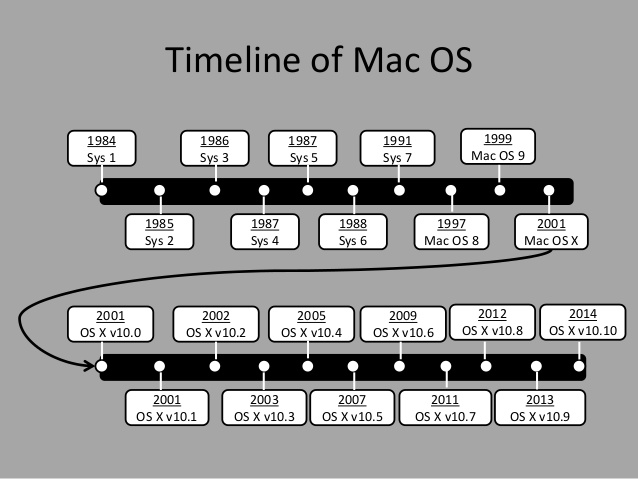
\includegraphics[scale=0.6]{img/mactl.jpg}
\caption{Historial de Versiones Mac OS}
\label{fig:dis2}
\end{figure}
\end{center}

\begin{center}
\begin{figure}[H]
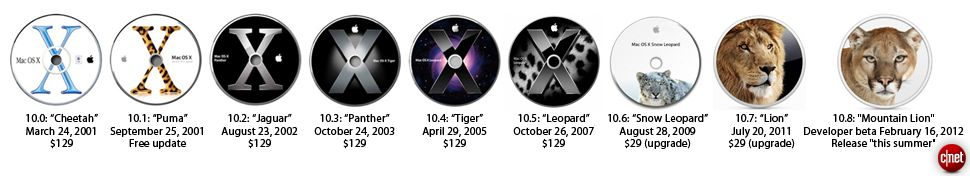
\includegraphics[scale=0.4]{img/tl.jpg}
\caption{Versiones con Nombre MacOS}
\label{fig:dis2}
\end{figure}
\end{center}
\section{Proceso de Instalación}
El proceso para realizar la instalación de este sistema operativo  para este caso es obtener los instaladores y recursos del link compartido por el \fnurl{profesor}{https://drive.google.com/drive/folders/0B4oI2NCmjimgNlg4T2FYVzBtVGs}, realizamos el proceso pertinente de descarga y revision de los archivos como se muestra en la siguiente figura : 

\begin{center}
\begin{figure}[H]
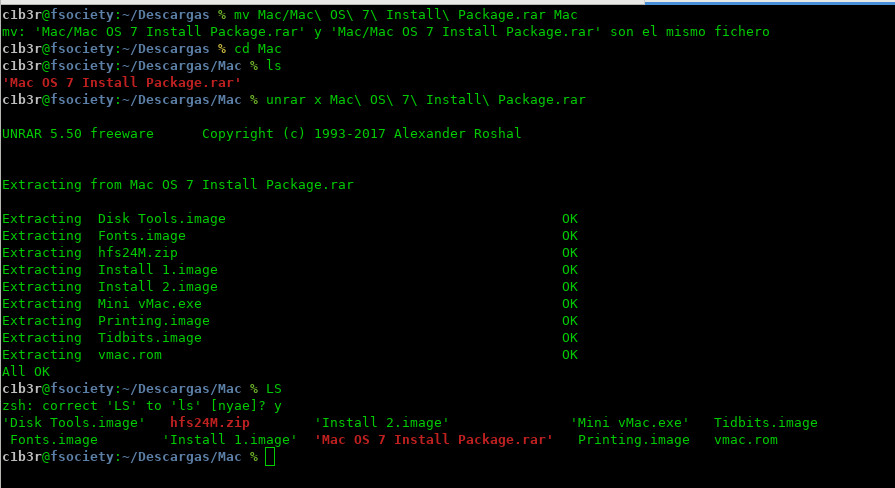
\includegraphics[scale=0.4]{img/mac.jpg}
\caption{detalles de instalador, recursos compartidos por profesor}
\label{fig:installer}
\end{figure}
\end{center}
Al descomprimir los archivos notamos que hay varios archivos \textbf{.image} desafortunadamente, estos archivos con muchas configuraciones realizadas no son detectados adecuadamente por las unidades de disquete de virtualbox, pero en el paque se provee 
un archivo ejecutable que lo que viene precargado con un bootloader y con la simulacion de las configuraciones de hardware para el MacOS X 7, es de decir que esta misma version es la que se encuentra en \fnurl{JamesFriend}{https://jamesfriend.com.au/pce-js/} un bootloader escrito puramente en javascript poniendo a disposicion de todas las personas probar y manipular una version legacy de MacOs.

\begin{figure}[H]
 	\centering
   	\subfloat[Ejecucion de MiniVmac.exe wine utils, linux]{\label{fig:cmd7}{
   		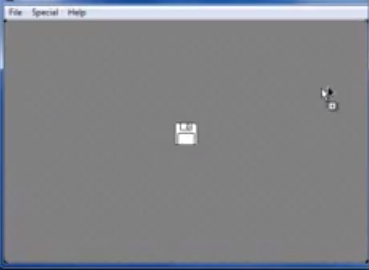
\includegraphics[width=0.68\textwidth]{img/1.png}
   		}}
	\subfloat[Install Wizard, Easy Install.]{\label{fig:cmd8}{
   		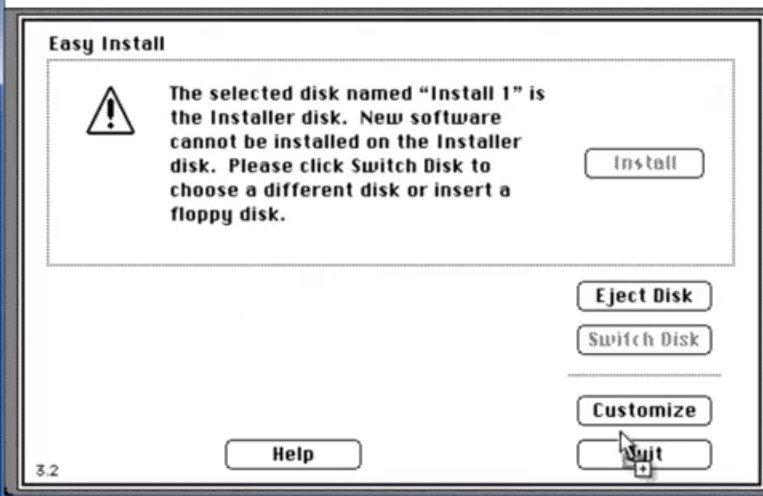
\includegraphics[width=0.68\textwidth]{img/2.png}
        }}
       \hfill
	\subfloat[Insercion de Imagen 1]{\label{fig:cmd3}{
   		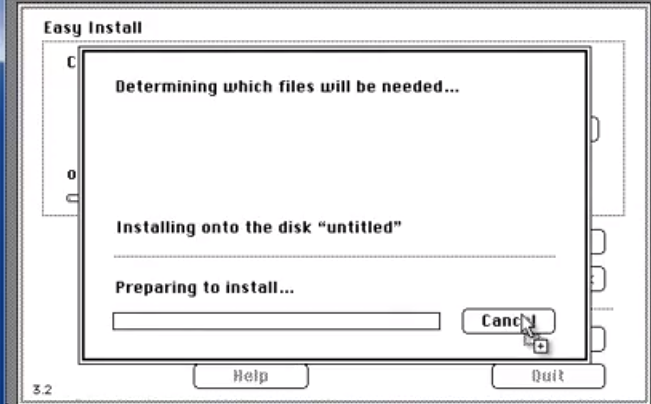
\includegraphics[width=0.68\textwidth]{img/3.png}
        }}
	\subfloat[Proceso de Instalacion Imagen 1 iniciado]{\label{fig:cmd9}{
   		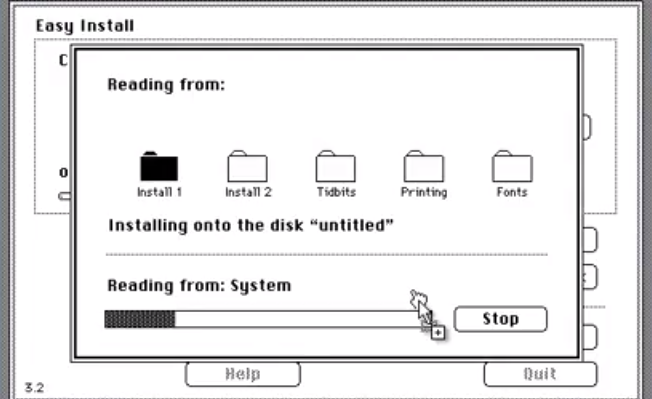
\includegraphics[width=0.68\textwidth]{img/4.png}
        }}
        \hfill
	\subfloat[Insercion de Imagen 2]{\label{fig:cmd10}{
   		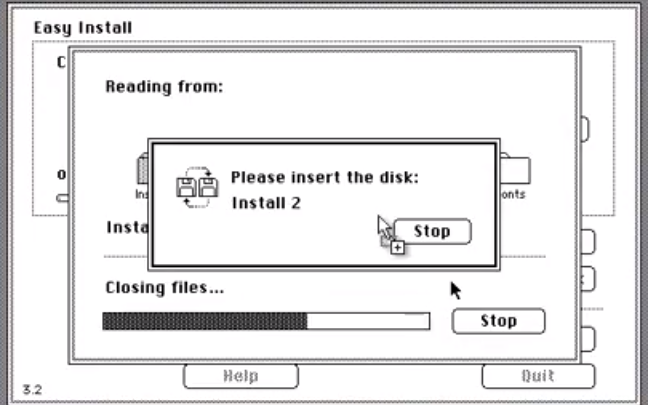
\includegraphics[width=0.68\textwidth]{img/5.png}
        }}
	\subfloat[Instalacion de Tidibits package.]{\label{fig:particiones}{
   		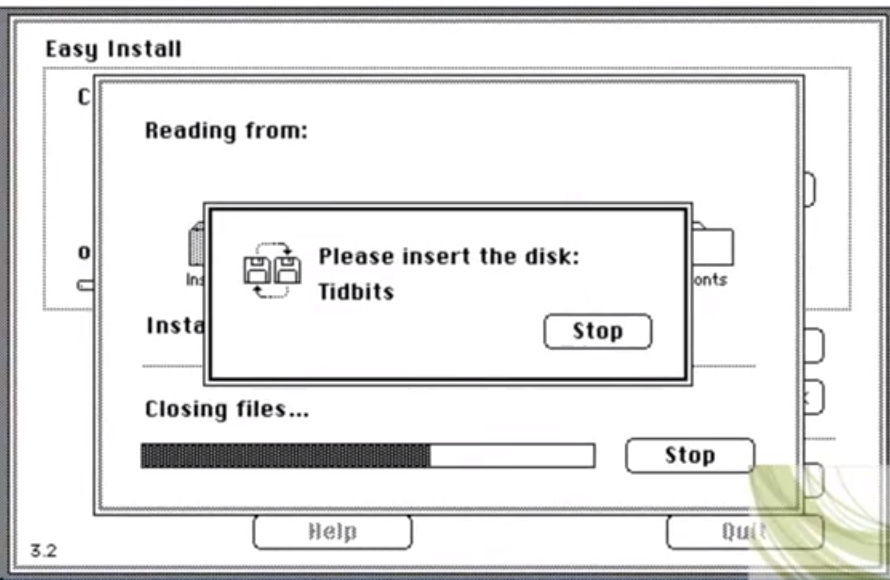
\includegraphics[width=0.68\textwidth]{img/6.png}
        }}
	\caption{Configuración inicial de instalación}
\end{figure}

Al realizar el proceso de instalacion una vez iniciamos el sistema operativo nos damos cuenta que su version especifica es 7.0.1 Por otra parte es posible observar que este sistema operativo es bastante obsoleto pero base de los sistemas operativos de la linea de mac actuales, se aprecia que tiene aplicaciones novedosas para su tiempo como MacPaint, MacDraw, y Kid Pix para hacer tareas de diseño. 
\begin{center}
\begin{figure}[H]
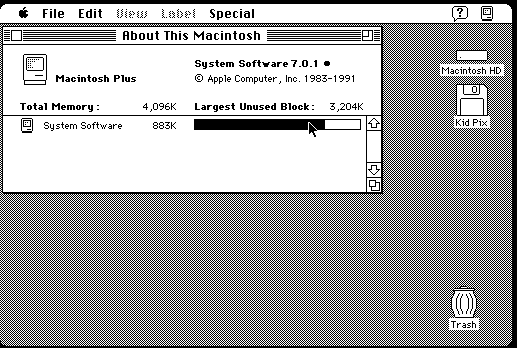
\includegraphics[scale=0.6]{img/mac1.png}
\caption{Historial de Versiones Mac OS}
\label{fig:dis2}
\end{figure}
\end{center}
\begin{center}
\begin{figure}[H]
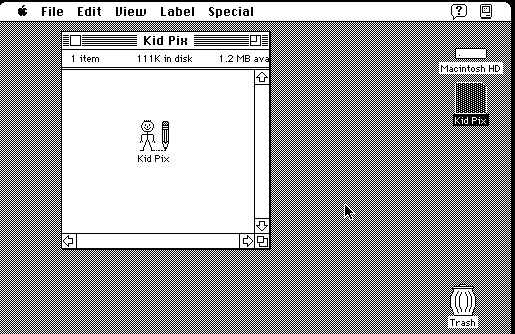
\includegraphics[scale=0.6]{img/mac2.png}
\caption{Historial de Versiones Mac OS}
\label{fig:dis2}
\end{figure}
\end{center}
\section{Manejo de Archivos, Shell}
De esta versión de mac os x el manejo de archivos es posible realizar con un adminsitrador de archivos rudimentario teniendo en cuenta el proceso y gestion de este tipo de sistema operativo como se ve en la fig \ref{fig:io}. 

Desafortunadamente, para la simulacion de vmac.exe no fue posible acceder a ninguna terminal o shell, ni si quiera las utilidades presentes en el simulador del navegador. 

\section{Estructura del Sistema Operativo}
La arquitectura del sistema operativo MacOS se sustenta en cuatro pilares de diseño ellos son ::
\begin{itemize}
\item La base o kernel del sistema, encargado de interactuar con el hardware de la máquina, es decir, de acceder a recursos como la memoria, unidades de almacenamiento.
\item El sistema gráfico, formado por la combinación de tres componentes clave, llamados Quartz, QuickTime y OpenGL.
\item Un entorno de programación y desarrollo que permite exprimir al máximo las nuevas posibilidades del sistema, portar con facilidad las aplicaciones ya existentes y emular el entorno operativo actual: Cocoa, Carbon y Classic.
\item  Una interfaz de usuario totalmente renovada, con aspecto, rendimiento, usabilidad y funcionalidades fuera de lo normal, que se ha convertido en el estandarte del nuevo sistema: Aqua.
\end{itemize}
POSIX / BSD

Provee al OS de la personalidad propia del sistema Macintosh.
Manejo de las API encargadas del sistema de ficheros:

\begin{enumerate}
\item Diseño mejorado del VFS
\item Soporta múltiples formatos de ficheros (HFS, USF, HFS Plus).
\item Permite compartir ficheros NFS, y da servicio a los servicios de Telnet, FTP, esto es algo común en todos los sistemas UNIX.
\item Darwin incorpora la pila (stack) de protocolos para redes de BSD, la que es usada por gran cantidad de equipos que trabajan con el protocolo TCP/IP.
\item Soporte multiprocesador
\item Soporte de AppleTalk.
\item Todo convenientemente actualizado para la nueva versión de protocolo IP, conocida por Ipv6.
\end{enumerate}

El kernel Mach 3.0, permite el uso de varios procesadores trabajando en paralelo. Aunque hoy por hoy, el OS X no está capacitado al 100\% para el uso de esta funcionalidad, en breve se cree que se podrá implementar del todo en el OS, ya que su kernel esta preparado para ello.

\begin{center}
\begin{figure}[H]
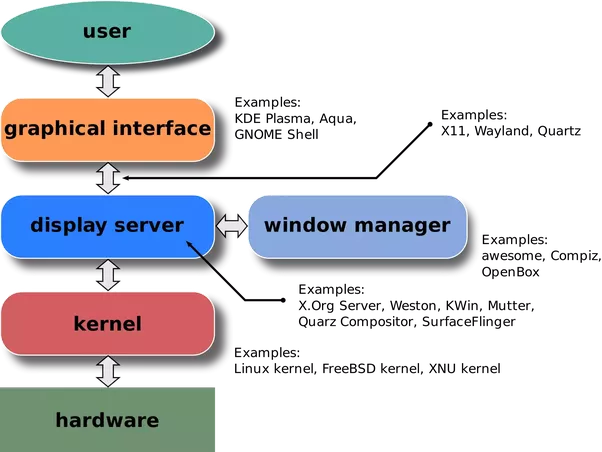
\includegraphics[scale=0.4]{img/main.jpg}
\caption{Estructura y gestión de sistema operativo, Apple, Linux, Unix. Con los diferentes servicios}
\label{fig:io}
\end{figure}
\end{center} 
\begin{center}
\begin{figure}[H]
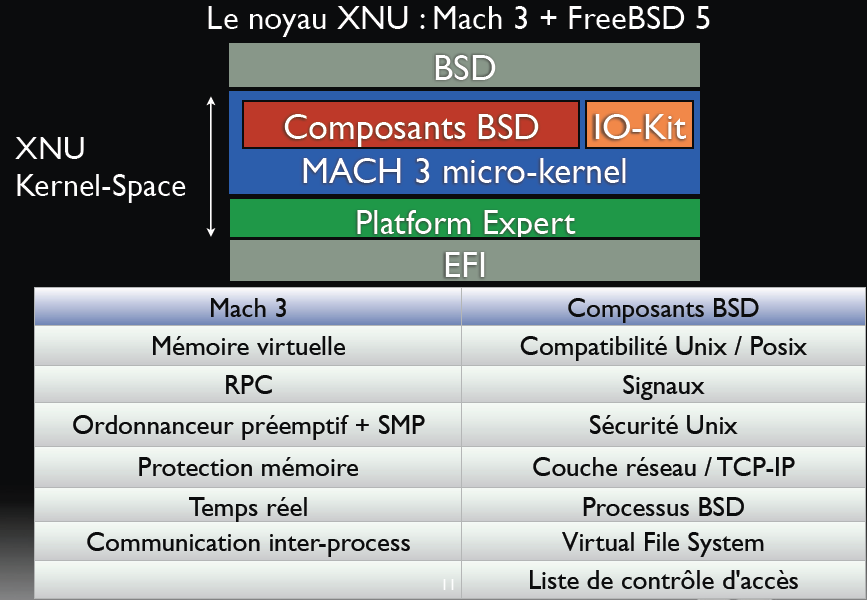
\includegraphics[scale=0.4]{img/xnu.png}
\caption{Configuración y Estructura de Xnu Mac OS}
\label{fig:dis2}
\end{figure}
\end{center}

\section{Clasificación}
Este sistema operativo se clasifica como : 
\begin{itemize}
\item Multiproceso 
\item Multiusuario
\item Multitarea
\item Propósito general
\item Micronúcleo
\item Cerrado  en su  desarrollo
\end{itemize}
\section{Referencias}
\begin{itemize}
\item  \hyperref[https://en.wikipedia.org/wiki/XNU]{Xnu Kernel Description,https://en.wikipedia.org/wiki/XNU}
\item \hyperref[https://en.wikipedia.org/wiki/MacOS_version_history]{Historia Mac OS X, https://en.wikipedia.org/wiki/MacOS\_version\_history}
\item \hyperref[https://jamesfriend.com.au/pce-js/pce-js-apps/]{James Friend, Vmac emulator https://jamesfriend.com.au/pce-js/pce-js-apps/}
\end{itemize}
\end{document}